\documentclass[tikz]{standalone}
\begin{document}
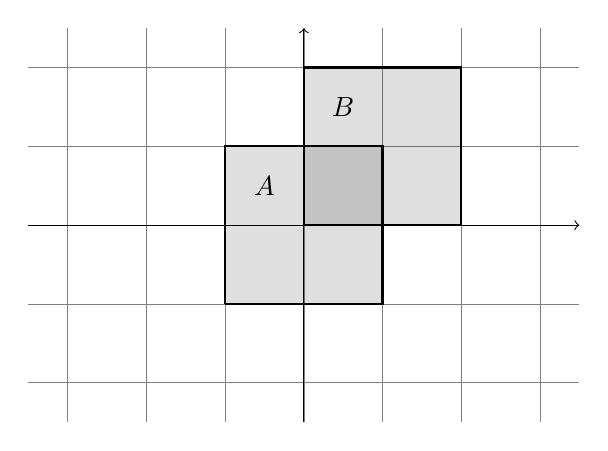
\begin{tikzpicture}
  \draw[help lines] (-3.5,-2.5) grid (3.5,2.5);
  \draw [->] (-3.5,0) -- (3.5,0);
  \draw [->] (0,-2.5) -- (0,2.5);
  \draw[thick, fill=black, fill opacity=0.125] (-1,-1) -- (1,-1) -- (1,1) -- (-1, 1) -- (-1, -1);
  \node at (-0.5,0.5) {$A$};
  \draw[thick, fill=black, fill opacity=0.125] (0,0) -- (2,0) -- (2,2) -- (0, 2) -- (0, 0);
  \node at (0.5,1.5) {$B$};
\end{tikzpicture}
\end{document}
